\documentclass[12pt, titlepage]{article}

\usepackage{amsmath, mathtools}

\usepackage[round]{natbib}
\usepackage{amsfonts}
\usepackage{amssymb}
\usepackage{graphicx}
\usepackage{colortbl}
\usepackage{xr}
\usepackage{hyperref}
\usepackage[normalem]{ulem}
\usepackage{longtable}
\usepackage{xfrac}
\usepackage{tabularx}
\usepackage{float}
\usepackage{siunitx}
\usepackage{booktabs}
\usepackage{multirow}
\usepackage[section]{placeins}
\usepackage{caption}
\usepackage{fullpage}
\usepackage{soul}

\hypersetup{
bookmarks=true,     % show bookmarks bar?
colorlinks=true,       % false: boxed links; true: colored links
linkcolor=red,          % color of internal links (change box color with linkbordercolor)
citecolor=blue,      % color of links to bibliography
filecolor=magenta,  % color of file links
urlcolor=cyan          % color of external links
}

\usepackage{array}

\externaldocument{../../SRS/SRS}

\newcounter{mnum}
\newcommand{\mthemnum}{M\themnum}
\newcommand{\mref}[1]{M\ref{#1}}

%% Comments

\usepackage{color}

\newif\ifcomments\commentstrue %displays comments
%\newif\ifcomments\commentsfalse %so that comments do not display

\ifcomments
\newcommand{\authornote}[3]{\textcolor{#1}{[#3 ---#2]}}
\newcommand{\todo}[1]{\textcolor{red}{[TODO: #1]}}
\else
\newcommand{\authornote}[3]{}
\newcommand{\todo}[1]{}
\fi

\newcommand{\wss}[1]{\authornote{blue}{SS}{#1}} 
\newcommand{\plt}[1]{\authornote{magenta}{TPLT}{#1}} %For explanation of the template
\newcommand{\an}[1]{\authornote{cyan}{Author}{#1}}

%% Common Parts

\newcommand{\progname}{ProgName} % PUT YOUR PROGRAM NAME HERE
\newcommand{\authname}{Team \#, Team Name
\\ Student 1 name
\\ Student 2 name
\\ Student 3 name
\\ Student 4 name} % AUTHOR NAMES                  

\usepackage{hyperref}
    \hypersetup{colorlinks=true, linkcolor=blue, citecolor=blue, filecolor=blue,
                urlcolor=blue, unicode=false}
    \urlstyle{same}
                                


\begin{document}

\title{Module Interface Specification for Hairesthetics}

\author{Team 18 \\ Charlotte Cheng
        \\ Marlon Liu
        \\ Senni Tan
        \\ Qiushi Xu
        \\ Hongwei Niu
        \\ Bill Song
}

\date{\today}

\maketitle

\pagenumbering{roman}

\section{Revision History}

\begin{tabularx}{\textwidth}{p{3cm}p{2cm}X}
\toprule {\bf Date} & {\bf Version} & {\bf Notes}\\
\midrule
Jan 15 & 0.1 & Initial Draft\\
Jan 16 & 0.2 & Minor updates\\
Jan 17 & 1 & Rev0 MIS\\
Apr 1 & 2 & Final Doc Update\\
Apr 4 & 2.1 & Minor update to modules\\
\bottomrule
\end{tabularx}

~\newpage

\section{Symbols, Abbreviations and Acronyms}
\begin{tabular}{l l} 
  \toprule		
  \textbf{symbol} & \textbf{description}\\
  \midrule 
  ML & Machine Learning \\
  UI & User Interface\\
  AI & Artificial Intelligence \\
  AR & Augumented Reality \\
  App & Application \\
  API & Application programming interface\\
  REST & Representational state transfer\\
  RGB & Red, Green, Blue \\
  macOS & Operating system developed by Apple Inc \\
  MG & Module Guide \\
  MIS & Module Interface Specification \\
  \bottomrule
\end{tabular}\\
\newline
See SRS Documentation at \href{https://github.com/marlon4dashen/Hairesthetics/blob/main/docs/SRS/SRS.pdf}{/docs/SRS/SRS.pdf}

\newpage

\tableofcontents
\listoftables
\listoffigures

\newpage

\pagenumbering{arabic}

\section{Introduction}

The following document details the Module Interface Specifications for the Hairesthetics application. Hairesthetics is an application that simulates 3D hairstyles.

Complementary documents include the System Requirement Specifications
and Module Guide.  The full documentation and implementation can be
found at \url{https://github.com/marlon4dashen/Hairesthetics}. 

\section{Notation}

The structure of the MIS for modules comes from HoffmanAndStrooper1995,
with the addition that template modules have been adapted from
GhezziEtAl2003. The mathematical notation comes from Chapter 3 of
HoffmanAndStrooper1995. For instance, the symbol:= is used for a
multiple assignment statement and conditional rules follow the form $(c_1
\Rightarrow r_1 | c_2 \Rightarrow r_2 | ... | c_n \Rightarrow r_n )$.

The following table summarizes the primitive data types used by the modules. 

\begin{center}
\renewcommand{\arraystretch}{1.2}
\noindent 
\begin{tabular}{l l p{7.5cm}} 
\toprule 
\textbf{Data Type} & \textbf{Notation} & \textbf{Description}\\ 
\midrule
character & char & a single symbol or digit\\
integer & $\mathbb{Z}$ & a number without a fractional component in (-$\infty$, $\infty$) \\
natural number & $\mathbb{N}$ & a number without a fractional component in [1, $\infty$) \\
real & $\mathbb{R}$ & any number in (-$\infty$, $\infty$)\\
\bottomrule
\end{tabular} 
\end{center}

\noindent
The specification of our modules uses some derived data types: sequences, strings, and tuples. Sequences are lists filled with elements of the same data type. Strings are sequences of characters. Tuples contain a list of values, potentially of different types. In addition, our modules use functions, which are defined by the data types of their inputs and outputs. Local functions are described by giving their type signature followed by their specification.

\section{Module Decomposition}

This section provides an overview of the module design. Modules are summarized
in a hierarchy decomposed by secrets in Table \ref{TblMH}. The modules listed
below, which are leaves in the hierarchy tree, are the modules that will
actually be implemented.

\begin{description}
\item [\refstepcounter{mnum} \mthemnum \label{mHH}:] \sout{Controller Module} \textcolor{red}{App Module}
\item [\refstepcounter{mnum} \mthemnum \label{mHH}:] \textcolor{red}{Server Module}
\item [\refstepcounter{mnum} \mthemnum \label{mHH}:] Hair Color Module
\item [\refstepcounter{mnum} \mthemnum \label{mHH}:] \textcolor{red}{Worker Module}
\item [\refstepcounter{mnum} \mthemnum \label{mHH}:] \textcolor{red}{Image Worker Module}
\item [\refstepcounter{mnum} \mthemnum \label{mHH}:] Salon Recommendation Module
\item [\refstepcounter{mnum} \mthemnum \label{mHH}:] \textcolor{red}{Hair Artist Module}
\item [\refstepcounter{mnum} \mthemnum \label{mHH}:] \textcolor{red}{Model Utils Module}
\item [\refstepcounter{mnum} \mthemnum \label{mHH}:] \textcolor{red}{Image Utils Module}
\item [\refstepcounter{mnum} \mthemnum \label{mHH}:] Hair Color View Module
\item [\refstepcounter{mnum} \mthemnum \label{mHH}:] Hair Style View Module
\item [\refstepcounter{mnum} \mthemnum \label{mHH}:] Salon Recommendation View Module
\item [\refstepcounter{mnum} \mthemnum \label{mHH}:] Home View Module
\item [\refstepcounter{mnum} \mthemnum \label{mHH}:] \sout{Error View Module} \textcolor{red}{Footer Module}
\item [\refstepcounter{mnum} \mthemnum \label{mHH}:] \sout{Camera Module} \textcolor{red}{NavBar Module}
\item [\refstepcounter{mnum} \mthemnum \label{mHH}:] \sout{Launch View Module} \textcolor{red}{AR Canvas Module}
\item [\refstepcounter{mnum} \mthemnum \label{mHH}:] \textcolor{red}{HairModel Module}
\item [\refstepcounter{mnum} \mthemnum \label{mHH}:] \textcolor{red}{ThreeFiber Helper Module}
\end{description}

\begin{table}[H]
\centering
\begin{tabular}{p{0.3\textwidth} p{0.6\textwidth}}
\toprule
\textbf{Level 1} & \textbf{Level 2}\\
\midrule

{Hardware-Hiding Module} & \sout{M13} \textcolor{red}{M1} \\
\midrule

\multirow{7}{0.3\textwidth}{Behaviour-Hiding Module}
& \sout{M1}\\
& M2\\
& M3\\
& M4\\
& M5\\
& \textcolor{red}{M6} \\
& \textcolor{red}{M7} \\
& M10\\
& M11\\
& \textcolor{red}{M12} \\
& \textcolor{red}{M13} \\
& M14\\
& \textcolor{red}{M15} \\
& \textcolor{red}{M16} \\
& \textcolor{red}{M17} \\
\midrule

\multirow{2}{0.3\textwidth}{Software Decision Module} 
& \sout{M6} \\  
& \sout{M7}\\
& \textcolor{red}{M8} \\
& \textcolor{red}{M9}\\
& \textcolor{red}{M18} \\
\bottomrule

\end{tabular}
\caption{Module Hierarchy}
\label{TblMH}
\end{table}



\subsection{UML Diagram}
\newpage

\begin{center}
\begin{figure}[]
% \graphicspath{ {component_diagram.jpg} }
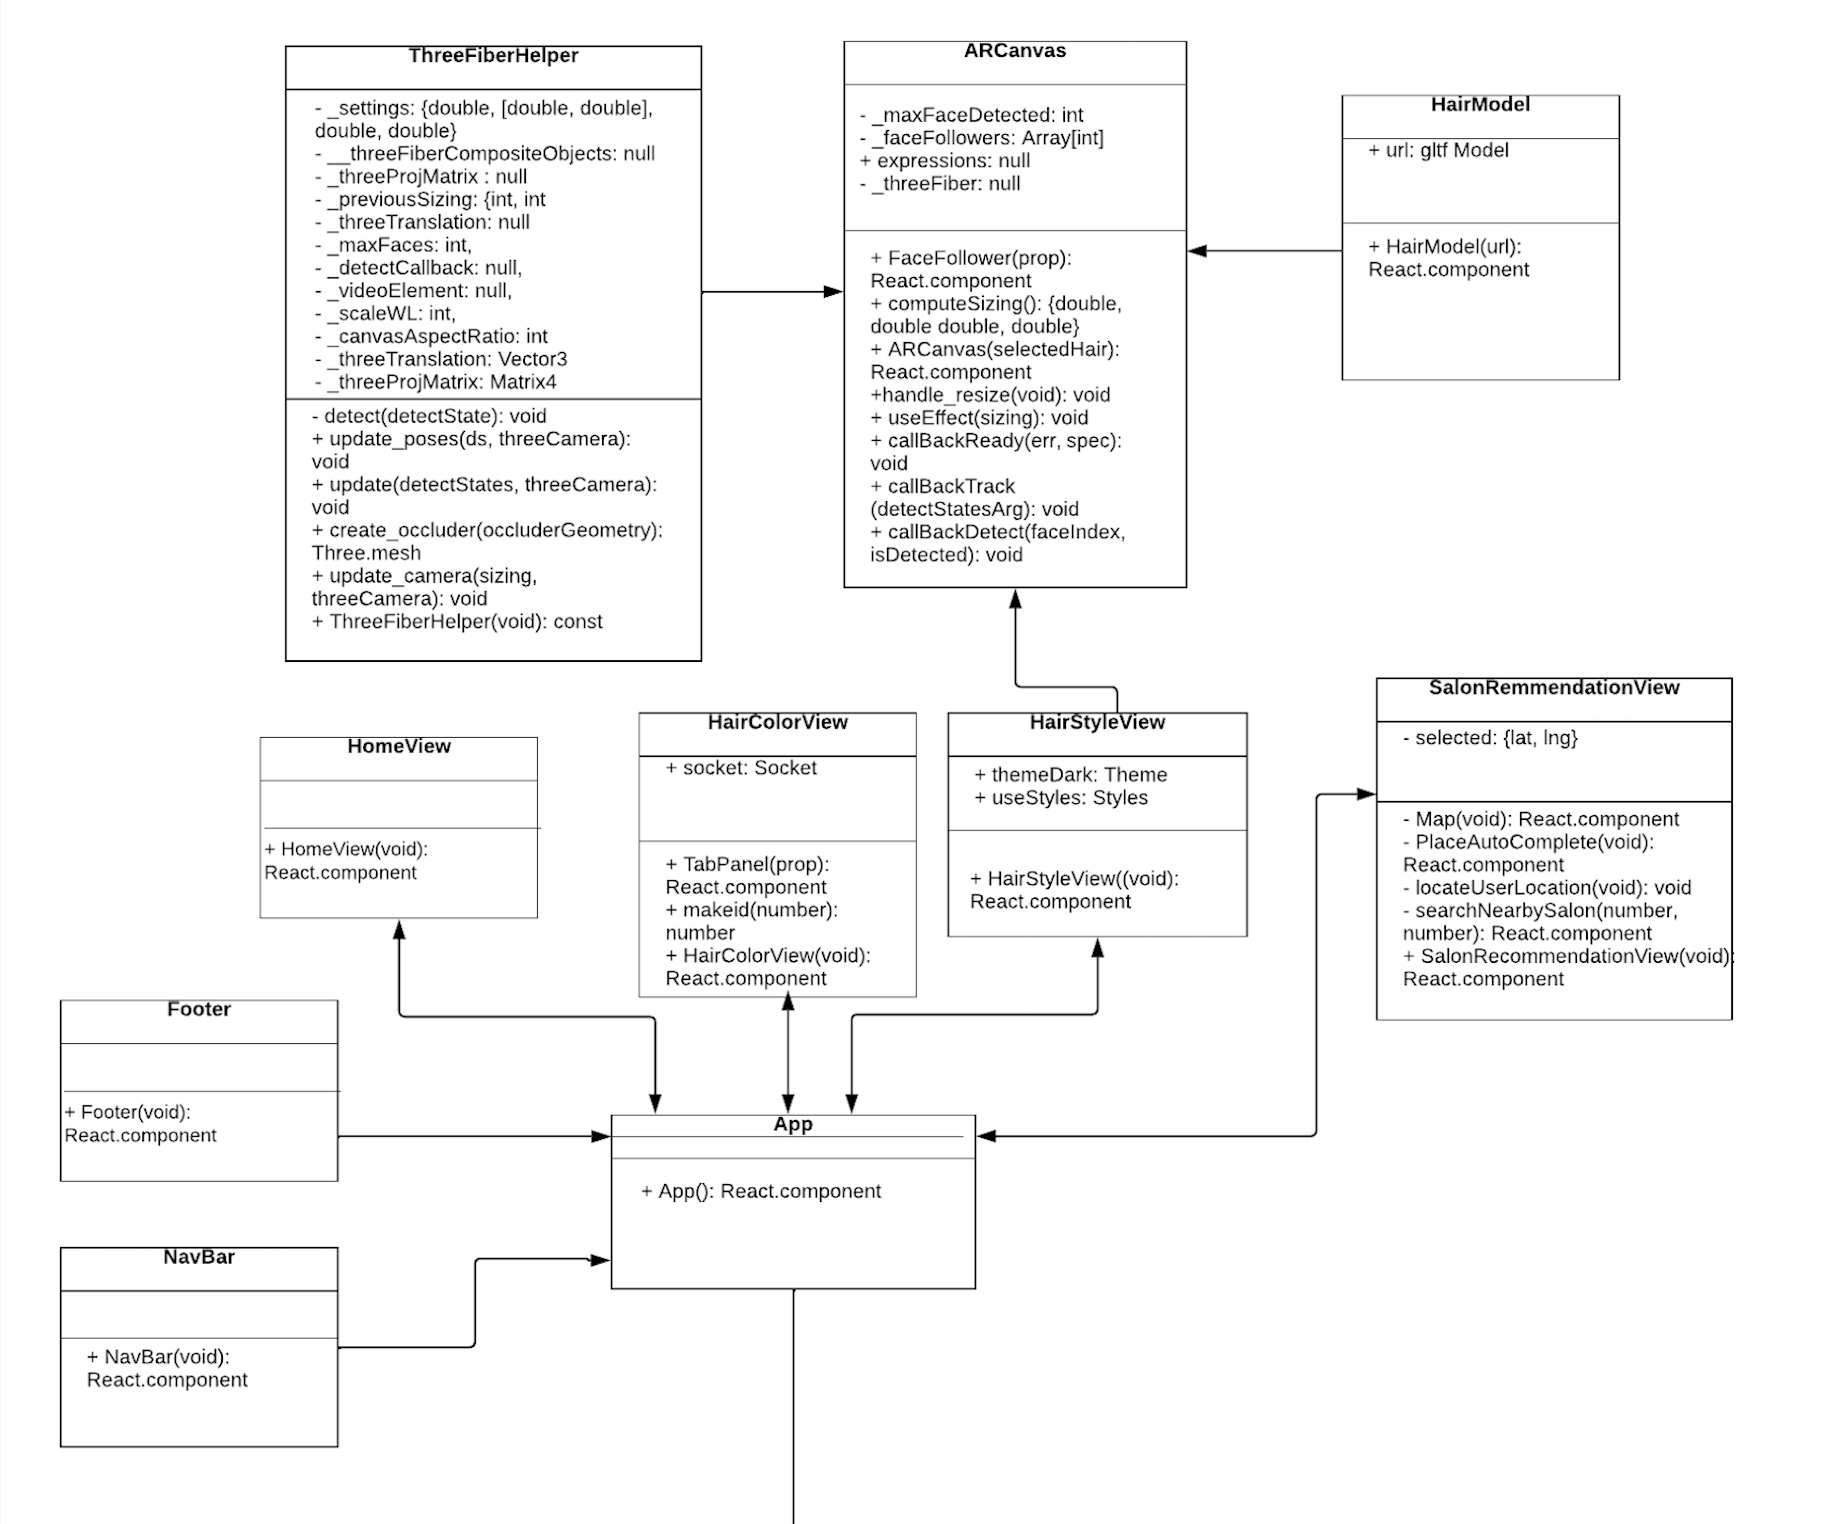
\includegraphics[width=0.8\textwidth, scale=1.5, keepaspectratio]{Design/SoftArchitecture/uml1.png}
\caption{UML Diagram Part 1}
\label{FigUH} 
\end{figure}
\end{center}

\begin{center}
\begin{figure}[]
% \graphicspath{ {component_diagram.jpg} }
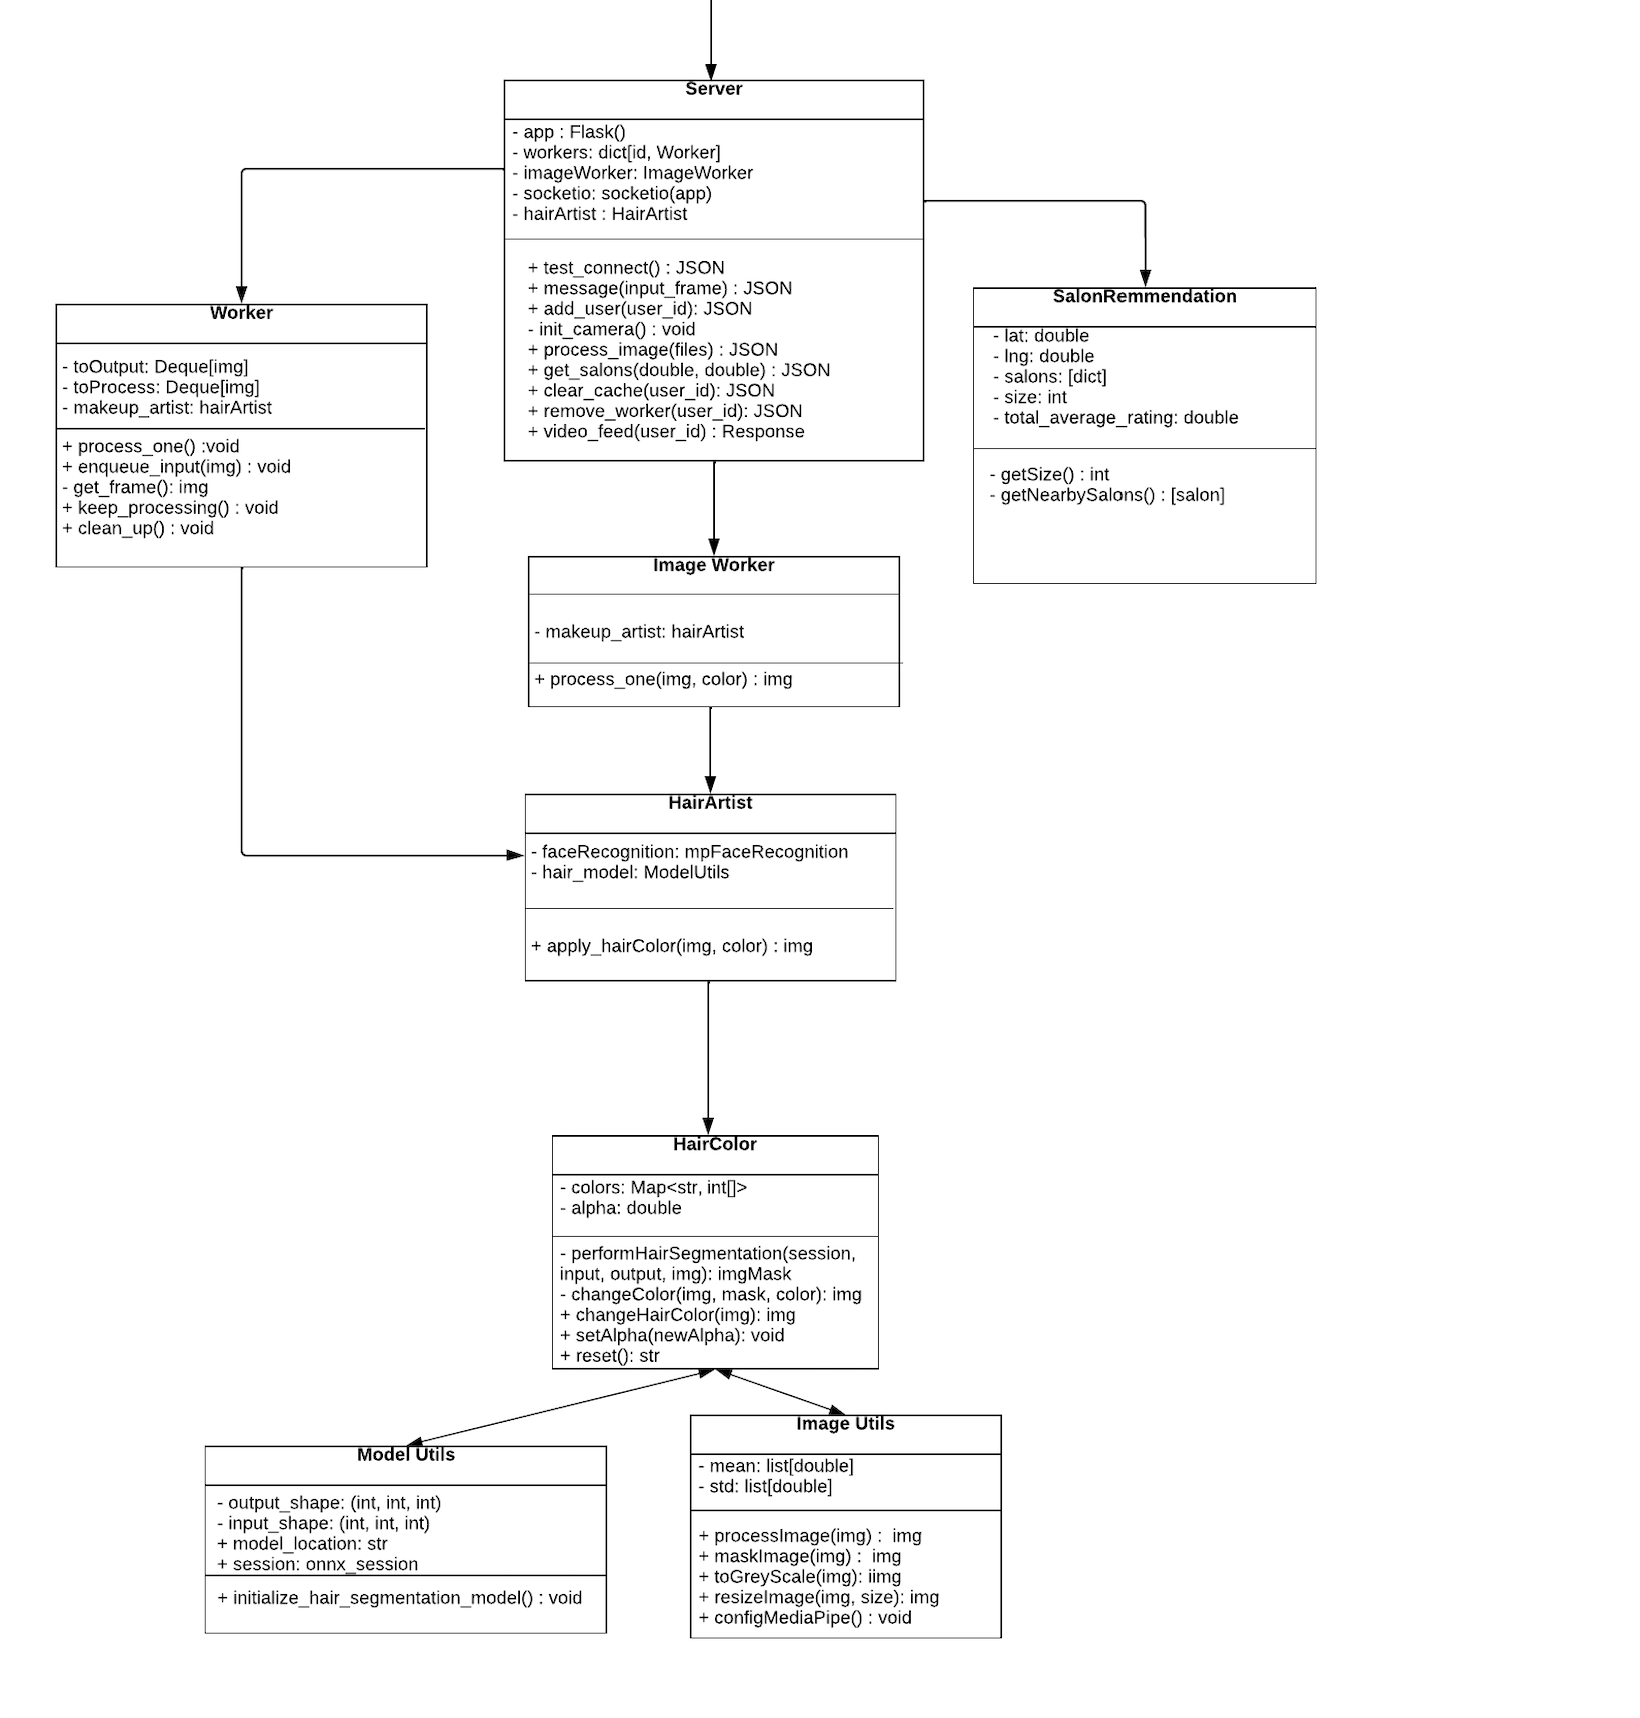
\includegraphics[width=0.8\textwidth, scale=1.5, keepaspectratio]{Design/SoftArchitecture/uml2.png}
\caption{UML Diagram Part 2}
\label{FigUH} 
\end{figure}
\end{center}

~\newpage

\section{\sout{MIS of Controller Module}\textcolor{red}{App Module}}

\subsection{Module}
M1 - App Module \\
Abstract Data Type Module

\subsection{\textcolor{red}{Uses}}
Server Module (M2) \\
HairColorView (M10) \\
HairStyleView (M11) \\
SalonRecommendationView (M12) \\
HomeView (M13) \\
Footer Module (M14) \\
NavBar Module (M15) \\

\subsection{Syntax}

\subsubsection{Exported Constants}

\subsubsection{Exported Access Programs}

\begin{center}
\begin{tabular}{p{5cm} p{3cm} p{3cm} p{2cm}}
\hline
\textbf{Name} & \textbf{In} & \textbf{Out} & \textbf{Exceptions} \\
\hline
App & - & - & - \\
\hline
\end{tabular}
\end{center}

\subsection{Semantics}

\subsubsection{State Variables}
\sout{hairColorScreen := HairColorView \\
hairStyleScreen := HairStyleView \\
salonRecomScreen := SalonRecommendationView \\
camera := Camera \\
homeScreen := HomeView \\
launchScreen := launchView \\
errorScreen := errorView \\
facialRecognitionModel := FacialRecognition \\
hairColorModel := HairColor \\
hairStyleModel := HairStyle \\
salonRecommendationModel := SalonRecommendation \\
currentView := homeScreen}

\subsubsection{Environment Variables}

\subsubsection{Assumptions}

\subsubsection{\textcolor{red}{Access Routine Semantics}}

\noindent App():
\begin{itemize}
\item transition: \\
app := react.component() 
\item output: 
\item exception:
\end{itemize}

\subsubsection{\textcolor{red}{Local Functions}}


\color{red}
\newpage
\section{\textcolor{red}{MIS of Server Module}}
\subsection{Module}
M2 - Server\\
Abstract Object Module

\subsection{Uses}
Worker (M4) \\
Hair Artist (M7) \\
Salon Recommendation (M6) \\
Flask \\
SocketIO 

\subsection{\textcolor{red}{Syntax}}

\subsubsection{Exported Constants}
\subsubsection{Exported Access Programs}

\begin{center}
\begin{tabular}{p{4cm} p{3cm} p{4cm} p{4cm}}
\hline
\textbf{Name} & \textbf{In} & \textbf{Out} & \textbf{Exceptions} \\
\hline
test\_connect &  & JSON & \\
message & JSON &  &  \\
add\_user & int & JSON & \\
init\_camera &  &  & \\
process\_images & File & JSON & \\
get\_salons & double, double & JSON & \\
clear\_cache & int & JSON & KeyError\\
remove\_worker & int & JSON & KeyError\\
video\_feed & int & JSON & KeyError\\
\hline
\end{tabular}
\end{center}

\subsection{\textcolor{red}{Semantics}}

\subsubsection{State Variables}
app := Flask() \\
workers := dict() \\
imageWorker := null \\
socketio := SocketIO(app) \\
hairArtist := null \\
salonRecommendation := null

\subsubsection{Environment Variables}

\subsubsection{Assumptions}

\subsubsection{\textcolor{red}{Access Routine Semantics}}
\noindent \textcolor{red}{test\_connect()}:
\begin{itemize}
\item transition:
\item output: \\
return output - JSON with 200 status connection success
\item exception: 
\end{itemize}

\noindent \textcolor{red}{message(img, color, user\_id)}:
\begin{itemize}
\item transition: worker[user\_id].enqueue\_input = (img, color)
\item output: JSON with 200 status success
\item exception: 
\end{itemize}

\noindent \textcolor{red}{add\_user(user\_id)}:
\begin{itemize}
\item transition: 
hairArtist = HairArtist() if hairArtist == none \\
worker[user\_id] = Worker(hairArtist)
\item output: JSON with 200 status success
\item exception: 
\end{itemize}

\noindent \textcolor{red}{init\_camera(user\_id)}:
\begin{itemize}
\item transition: imageWorker = imageWorker(hairArtist)
\item output: JSON with 200 status success
\item exception: 
\end{itemize}

\noindent \textcolor{red}{process\_images(File, color, user\_id)}:
\begin{itemize}
\item transition: res = imageWorker.process\_one(files.toImage(), color)
\item output: JSON with processed frame status 200 success
\item exception: 
\end{itemize}

\noindent \textcolor{red}{get\_salons(lat, lng)}:
\begin{itemize}
\item input: lat - latitude in double, lng - longitude in double
\item transition: \\
salonRecommendation = salonRecommendation(lat, lng) \\
salons = salonRecommendation.get\_nearby\_salons()
\item output: salons - JSON with nearby salon informations and 200 status code
\item exception: 
\end{itemize}

\noindent \textcolor{red}{clear\_cache(user\_id)}:
\begin{itemize}
\item transition: \\
if user\_id exists: \\
workers[user\_id].clean\_up()
\item output: JSON with 200 status code success
\item exception: 
\end{itemize}

\noindent \textcolor{red}{remove\_worker(user\_id)}:
\begin{itemize}
\item transition: \\
if user\_id exists: \\
delete workers[user\_id]
\item output: JSON with 200 status code success
\item exception: 
\end{itemize}

\noindent \textcolor{red}{video\_feed(user\_id)}:
\begin{itemize}
\item transition: \\
if user\_id exists: \\
resp = gen(user\_id)
\item output: Response with form data containing the processed frames
\item exception: 
\end{itemize}

\subsubsection{Local Functions}
The generator function that generates the frame for different users\\ 
\textcolor{red}{gen(user\_id)}: 
\begin{itemize}
    \item transition: frame = worker[user\_id].get\_frame()
    \item output: yield formdata containing the frame
\end{itemize}
\color{black}

\newpage
\section{MIS of Hair Color Module}
\subsection{Module}
M3 - HairColor Module\\
Abstract Object Module

\subsection{Uses}
\textcolor{red}{Model Utils (M8)} \\
\textcolor{red}{Image Utils (M9)} \\
\sout{MLModel (M6)} \\
\sout{Utility (M7)}

\subsection{Syntax}

\subsubsection{Exported Constants}
\subsubsection{Exported Access Programs}

\begin{center}
\begin{tabular}{p{4cm} p{3cm} p{4cm} p{4cm}}
\hline
\textbf{Name} & \textbf{In} & \textbf{Out} & \textbf{Exceptions} \\
\hline
% performHairSegmentation & onnx\_session, list[int], list[int], image & image & InterruptException \\
% changeColor & image, image, string & image &  KeyErrorException\\
changeHairColor & image, string & image & KeyErrorException \\
setAlpha & double & & \\
reset & & string & \\
\hline
\end{tabular}
\end{center}

\subsection{Semantics}

\subsubsection{State Variables}
colors - Map$<$str, int[]$>$ - a mapping between the name of color and their rgb values \\
alpha - double - represents the ratio between the original image and the masked image \\ 
\textcolor{red}{min\_confidence\_value - double - the minimum confidence interval for machine learning model}

\subsubsection{Environment Variables}

\subsubsection{Assumptions}

\subsubsection{Access Routine Semantics}

\noindent changeHairColor(image, color):
\begin{itemize}
\item input: \\ image - the copy of an original image \\ color - the chosen hair color
\item transition: N/A
\item output:\\
hairModelSession = utility.getHairModel() \\
mask = performHairSegmentation(hairModelSession, hairModelSession.inputName, hairModelSession.output image) - the image where the hair detected by the model is masked. \\
outputImg = changeColor(image, mask, color) \\
return outputImg - an image where the hair color of each person is changed to the specified color
\item exception: InterruptException - the prediction and masking process is interrupted by the user
\end{itemize}

\noindent setAlpha(newAlpha):
\begin{itemize}
\item input: newAlpha - double - input alpha value for update
\item transition: alpha := newAlpha - update the alpha value
\item output: N/A
\item exception: N/A
\end{itemize}

\noindent reset():
\begin{itemize}
\item transition:
\item output: message $=>$ MLModel.reset(hair)
\item exception: 
\end{itemize}

\subsubsection{Local Functions}

\noindent performHairSegmentation(session, input, output, image):
\begin{itemize}
\item input: session  - the onnx inference session that contains the input model\\
input - list of integer - the input shape of the image\\
output - list of integer - the expected output shape\\
image - the copy of an original image
\item transition: N/A
\item output: mask - hair mask.
\begin{center}
\begin{figure}[H]
% \graphicspath{ {component_diagram.jpg} }

\includegraphics[width=0.5\textwidth]{Design/SoftDetailedDes/hair_mask.png}
\caption{Hair Mask after running the pre-trained hair segmentation model}
\label{Fig_UseHierarchy} 
\end{figure}
\end{center}
\item exception: KeyErrorException - the specified color is not in the color map
\end{itemize}

 \noindent changeColor(img, mask, color):
\begin{itemize}
\item input: img - the original image, mask - the masked image generated from hair segmentation, color - color's name as a string
\item transition: N/A
\item output: an image where the original image is mixed with the masked image.
\item exception: KeyErrorException - the specified color is not in the color map
\end{itemize}

\newpage
\section{\sout{MIS of Hair Style Module}}
\subsection{Module}
M9 - FacialRecognition\\
Abstract Object Module

\subsection{Uses}
MLModel (M6) \\
Utility (M7)

\subsection{Syntax}

\subsubsection{Exported Constants}
\subsubsection{Exported Access Programs}

\begin{center}
\begin{tabular}{p{4cm} p{3cm} p{4cm} p{4cm}}
\hline
\textbf{Name} & \textbf{In} & \textbf{Out} & \textbf{Exceptions} \\
\hline
computeHairCoordinate & list[double], list[double] & list[double] &  \\
computeRotationDegree & list[double], list[double] & list[double] &  \\
\hline
\end{tabular}
\end{center}

\subsection{Semantics}

\subsubsection{State Variables}

\subsubsection{Environment Variables}

\subsubsection{Assumptions}

\subsubsection{Access Routine Semantics}
\noindent computeHairCoordinate(basePosition, facialCoordinates):
\begin{itemize}
\item input: basePosition - the basePosition of the camera setting in a tuple \\
facialCoordinates - a list of coordinates of the facial features
\item transition: N/A
\item output: output the desired position to place the hairstyle centered at a coordinate, computed based on the base position and facial coordinates.
\item exception: InterruptException := action terminated by the user
\end{itemize}

\noindent computeRotationDegree(basePosition, facialCoordinates):
\begin{itemize}
\item input: basePosition - the basePosition of the camera setting in a tuple \\
facialCoordinates - a list of coordinates of the facial features
\item transition: N/A
\item output: output the desired rotation of the hairstyle when being placed on the user's face, computed based on the base position and facial coordinates.
\end{itemize}

\subsubsection{Local Functions}

\color{red}
\newpage
\section{\textcolor{red}{MIS of Worker Module}}
\subsection{\textcolor{red}{Module}}
M4 - Worker Module\\
Abstract Data Type Module

\subsection{\textcolor{red}{Uses}}
Hair Artist (M7) \\
Threading

\subsection{\textcolor{red}{Syntax}}

\subsubsection{Exported Constants}
\subsubsection{Exported Access Programs}

\begin{center}
\begin{tabular}{p{4cm} p{3cm} p{4cm} p{4cm}}
\hline
\textbf{Name} & \textbf{In} & \textbf{Out} & \textbf{Exceptions} \\
\hline
\_\_init\_\_ & HairArtist & Worker & \\
enqueue\_input & img, tuple & &   \\
get\_frame & & img &  \\
clean\_up & & & \\
\hline
\end{tabular}
\end{center}

\subsection{\textcolor{red}{Semantics}}

\subsubsection{\textcolor{red}{State Variables}}
thread - Thread - daemon thread processing images in the background \\ 
to\_process - Deque - Double ended queue that stores input images (FIFO) \\ 
to\_output - Deque - Double ended queue that stores output images (FIFO) \\ 
makeup\_artist - HairArtist - HairArtist instance that used for image processing 

\subsubsection{Environment Variables}

\subsubsection{Assumptions}

\subsubsection{\textcolor{red}{Access Routine Semantics}}
\noindent 
\textcolor{red}{\_\_init\_\_(hairArtist)}:
\begin{itemize}
\item input: hairArtist - HairArtist instance that used for image processing  \\
\item transition: \\
to\_process := Deque([])\\ 
to\_output := Deque([]) \\
makeup\_artist := hairArtist \\
thread = Thread(target=keep\_processing())
\item output:
\item exception:
\end{itemize}

\noindent 
\textcolor{red}{enqueue\_input(img, color)}:
\begin{itemize}
\item input: img - the input image from user  \\
tuple(color) - the input color to change hair to
\item transition: \\
to\_process.append((img, color))
\item output:
\item exception:
\end{itemize}

\noindent 
\textcolor{red}{get\_frame()}:
\begin{itemize}
\item input:
\item transition: \\
frame = to\_output.popleft(img)
\item output:\\
return - frame - processed image frame in order
\item exception:
\end{itemize}


\noindent 
\textcolor{red}{clean\_up()}:
\begin{itemize}
\item input:
\item transition: \\
to\_output.clear()\\ 
to\_process.clear() 
\item output:
\item exception:
\end{itemize}

\subsubsection{Local Functions}
\textcolor{red}{keep\_processing()}:  
\begin{itemize}
\item input:
\item transition: \\
while !to\_process().empty():\\
process\_one()
\item output:
\item exception:
\end{itemize}

\noindent
\textcolor{red}{process\_one()}: 
\begin{itemize}
\item input:
\item transition: \\
img, color = to\_process.popleft() \\
res = hair\_artist.apply\_hair\_color(img, color) \\
to\_output.append(res)
\item output:
\item exception:
\end{itemize}

\newpage
\section{\textcolor{red}{MIS of Image Worker Module}}
\subsection{\textcolor{red}{Module}}
M5 - Image Worker Module\\
Abstract Data Type Module

\subsection{\textcolor{red}{Uses}}
Hair Artist (M7)

\subsection{\textcolor{red}{Syntax}}

\subsubsection{Exported Constants}
\subsubsection{Exported Access Programs}

\begin{center}
\begin{tabular}{p{4cm} p{3cm} p{4cm} p{4cm}}
\hline
\textbf{Name} & \textbf{In} & \textbf{Out} & \textbf{Exceptions} \\
\hline
\_\_init\_\_ & HairArtist & ImageWorker & \\
process\_one & img, tuple & &  \\
\hline
\end{tabular}
\end{center}

\subsection{\textcolor{red}{Semantics}}

\subsubsection{\textcolor{red}{State Variables}}
makeup\_artist - HairArtist - HairArtist instance that used for image processing 

\subsubsection{Environment Variables}

\subsubsection{Assumptions}

\subsubsection{\textcolor{red}{Access Routine Semantics}}
\noindent 
\textcolor{red}{\_\_init\_\_(hairArtist)}:
\begin{itemize}
\item input: hairArtist - HairArtist instance that used for image processing  \\
\item transition: \\
to\_process := Deque([])\\ 
to\_output := Deque([]) \\
makeup\_artist := hairArtist \\
thread = Thread(target=keep\_processing())
\item output:
\item exception:
\end{itemize}


\noindent
\textcolor{red}{process\_one(img, color)}: 
\begin{itemize}
\item input: img - input image for hair segmentation \\ 
color - input color to change the hair \\
\item transition: \\
res = hair\_artist.apply\_hair\_color(img, color) \\
\item output:
\item exception:
\end{itemize}

\subsubsection{Local Functions}

\color{black}

 
\newpage
\section{MIS of Salon Recommendation Module} \label{Module} 

\subsection{Module}
M5: Salon Recommendation Module \\
Abstract Object Module


\subsection{Uses}


\subsection{Syntax}

\subsubsection{Exported Constants}

\subsubsection{\textcolor{red}{Exported Access Programs}}

\begin{center}
\begin{tabular}{p{4cm} p{3cm} p{4cm} p{4cm}}
\hline
\textbf{Name} & \textbf{In} & \textbf{Out} & \textbf{Exceptions} \\
\hline
get\_size & & int & \\
getNearbySalons & & list[salons] & \\
\hline
\end{tabular}
\end{center}

\subsection{Semantics}

\subsubsection{\textcolor{red}{State Variables}}

lat - double - latitude \\ 
lng - double - longitude \\ 
salons - list[dict] - contains the information of salons \\ 
size - int - size of nearby salons \\ 
total\_average\_rating - double - the average rating among all salons 

\subsubsection{Environment Variables}

\subsubsection{Assumptions}
\color{red}
\subsubsection{\textcolor{red}{Access Routine Semantics}}

\noindent \textcolor{red}{get\_size()}:
\begin{itemize}
\item input:
\item transition:  
\item output: \\ 
return - size - the size of nearby salons
\item exception: 
\end{itemize}

\noindent \textcolor{red}{getNearbySalons()}:
\begin{itemize}
\item input: 
\item transition: 
nearby\_salons = fetchNearbySalons(lat, lng) \\ 
foreach salon in nearby\_salons:
details = fetch\_place\_details \\
salons.append(details) \\ 
rank\_salons(salons)
\item output: \\
return - salons - the sorted nearby salon details list
\item exception: 
\end{itemize}


\subsubsection{\textcolor{red}{Local Functions}}
\noindent \textcolor{red}{fetchNearbySalons()}:
\begin{itemize}
\item input: 
\item transition: 
\item output: \\
return nearby\_salons - response from google map API. 
\item exception: 
\end{itemize}

\noindent \textcolor{red}{fetchPlaceDetails(place\_id)}:
\begin{itemize}
\item input: 
\item transition: 
\item output: \\
return salon\_info - the salon information with the given place\_id 
\item exception: 
\end{itemize}

\noindent \textcolor{red}{rank\_salons()}:
\begin{itemize}
\item input: 
\item transition: 
sort the salons with their average ratings generated by the bayesian algorithm
\item output: \\
\item exception: 
\end{itemize}


\newpage
\section{\textcolor{red}{MIS of Hair Artist Module}}
\subsection{\textcolor{red}{Module}}
M7 - HairArtist Module\\
Abstract Data Type Module

\subsection{\textcolor{red}{Uses}}
Model Utils Module (M8) \\
Image Utils Module (M9) \\ 
Hair Color Module (M3) 

\subsection{\textcolor{red}{Syntax}}

\subsubsection{Exported Constants}
\subsubsection{Exported Access Programs}

\begin{center}
\begin{tabular}{p{4cm} p{3cm} p{4cm} p{4cm}}
\hline
\textbf{Name} & \textbf{In} & \textbf{Out} & \textbf{Exceptions} \\
\hline
apply\_hair\_color & img, color & img & \\
\hline
\end{tabular}
\end{center}

\subsection{\textcolor{red}{Semantics}}

\subsubsection{\textcolor{red}{State Variables}}
face\_recognition - mediapipe instance of face recognition \\
hair\_model - ModelUtils instance with session that performs hair segmentation

\subsubsection{Environment Variables}

\subsubsection{Assumptions}

\subsubsection{\textcolor{red}{Access Routine Semantics}}

\noindent
\textcolor{red}{apply\_hair\_color(img, color)}: 
\begin{itemize}
\item input: img - input image for hair segmentation \\ 
color - input color to change the hair 
\item transition: \\
res = hair\_color.change\_hair\_color(img, color, hair\_model, face\_recognition)
\item output:
res - img - processed frame with hair color changed as desired
\item exception:
\end{itemize}

\subsubsection{Local Functions}

\color{black}
\section{\textcolor{red}{MIS of ModelUtils Module}}
\subsection{\textcolor{red}{Module}}
M8 - Model Utils Module\\
Abstract Data Type Module

\subsection{Uses}
Onnx (External Module) \\

\subsection{Syntax}

\subsubsection{Exported Constants}

\subsubsection{\textcolor{red}{Exported Access Programs}}

\begin{center}
\begin{tabular}{p{4cm} p{3cm} p{4cm} p{4cm}}
\hline
\textbf{Name} & \textbf{In} & \textbf{Out} & \textbf{Exceptions} \\
\hline
initialize\_hair\_segmentation\_model & & FileNotFoundException & \\
\hline
\end{tabular}
\end{center}

\subsection{\textcolor{red}{Semantics}}

\subsubsection{\textcolor{red}{State Variables}}
minConfidenceLevel - 0.5 - minimum confidence accuracy for output \\
inputShape - tuple - represent model input shape \\
outputShape - tuple - represent model output shape \\
modelFilePath - filePath (path to the pre-trained model) \\
model\_session - ML model with active session



\subsubsection{Environment Variables}

\subsubsection{Assumptions}

\subsubsection{\textcolor{red}{Access Routine Semantics}}
\color{red}
\noindent \textcolor{red}{initialize\_hair\_segmentation\_model()}:
\begin{itemize}
\item transition: \\
model\_session = onnx\_inference\_session(modelFilePath, minConfidenceLevel) \\ 
inputShape = model\_session.input\_shape \\ 
outputShape = model\_session.output\_shape \\ 
\item output: 
\item exception:
\end{itemize}
\color{black}

\subsubsection{Local Functions}

\newpage
\section{\textcolor{red}{MIS of Image Utils Module}}
\subsection{\textcolor{red}{Module}}
M9 - Utility Module\\
Library


\subsection{\textcolor{red}{Uses}}
OpenCV (External Module) \\
Numpy (External Module) \\
\color{red}
Pillow (External Module) \\ 
BytesIO (External Module) \\
base64 (External Module)
\color{black}

\subsection{\textcolor{red}{Syntax}}

\subsubsection{Exported Constants}
\subsubsection{Exported Access Programs}

\begin{center}
\begin{tabular}{p{4cm} p{3cm} p{4cm} p{4cm}}
\hline
\textbf{Name} & \textbf{In} & \textbf{Out} & \textbf{Exceptions} \\
\hline
processImage & image, list[int] & tensor & illegalArgumentException \\
maskImage & image, image & image  & illegalArgumentException \\
toGreyScale & image & image & \\
resizeImage & image, list[int] & image & illegalArgumentException \\
cv2\_image\_to\_base64 & img & string & illegalArgumentException & \\
base64\_to\_cv2\_image & string & img & illegalArgumentException & \\
\hline
\end{tabular}
\end{center}

\subsection{\textcolor{red}{Semantics}}

\subsubsection{State Variables}
mean - list[double] - the mean values of trained images, used to normalize the images \\
std - list[double] - the standard deviation values of trained images, used to normalize the images \\

\subsubsection{Environment Variables}

\subsubsection{Assumptions}

\subsubsection{Access Routine Semantics}
\noindent processImage(image, input\_size):
\begin{itemize}
\item input: image - the original input image in the form of 3-dimensional array, input\_size - a tuple represents the input size the ML model requires
\item transition: N/A
\item output: \\
OpenCV.convertColor(image, BGR2RGB) - convert the image to RGB format \\ resizeImage(image, input\_size) - convert image to input size \\
image = (image / 255 - mean) / std - normalize the image \\
Numpy.expandDimension(image, axis=0) - expand one dimension to a tensor \\
output a image tensor ready for process with the model
\item exception: illegalArgumentException - illegal input size for resizing
\end{itemize}

\noindent maskImage(original\_img, mask):
\begin{itemize}
\item input: original\_img - the original image in the form of 3-dimensional array, mask - the masked image in the form of 3-dimensional array with same dimension as original
\item transition: N/A
\item output: \\
OpenCV.bitwise\_or(original\_img, original\_img, mask) - apply masking to the original image with the given mask. \\
output a masked image.
\item exception: illegalArgumentException - original image has different size from the masked image.
\end{itemize}

\noindent toGreyScale(image):
\begin{itemize}
\item input: image - the input image to be converted to grey scale
\item transition: N/A
\item output: \\
OpenCV.convertColor(image, BGR2GRAY) - convert the input image to an grey scale image \\
output the greyscaled image
\item exception: 
\end{itemize}

\noindent resizeImage(image, shape):
\begin{itemize}
\item input: image - the input image \\
shape - a tuple represents the width / height to be reshaped into.
\item transition: N/A
\item output: \\
Numpy.reshape(image, shape) - reshape the image \\
output an reshaped image 
\item exception: illegalArgumentException - illegal input size for resizing
\end{itemize}
\color{red}
\noindent \textcolor{red}{cv2\_image\_to\_base64(image)}:
\begin{itemize}
\item input: image - the input image 
\item transition: N/A
\item output: \\
img = PIL.Image.fromarray(img) \\
base64.b64encode(img)
\item exception: illegalArgumentException - input array can not be transformed into image
\end{itemize}

\noindent \textcolor{red}{base64\_to\_cv2\_image(string)}:
\begin{itemize}
\item input: string - image string encoded in base64
\item transition: N/A
\item output: \\
str = base64.b64decode(string) \\ 
img = PIL.Image.open(str) \\
\item exception: illegalArgumentException - input string can not be transformed into image
\end{itemize}
\color{black}
\subsubsection{Local Functions}
None


\newpage
\section{MIS of Hair Color View Module} \label{Module} 
\subsection{Module}
M8 - HairColorView\\
Abstract Object Module

\subsection{Uses}
None

\subsection{Syntax}
\subsubsection{Exported Constants}
None

\subsubsection{Exported Access Programs}
\begin{center}
\begin{tabular}{p{4cm} p{3cm} p{4cm} p{4cm}}
\hline
\textbf{Name} & \textbf{In} & \textbf{Out} & \textbf{Exceptions} \\
\hline
\textcolor{red}{TabPanel} & \textcolor{red}{prop} & \textcolor{red}{React.component} & - \\
\textcolor{red}{makeid} & \textcolor{red}{number} & \textcolor{red}{number} & - \\
\textcolor{red}{HairColorView} & \textcolor{red}{void} & \textcolor{red}{React.component} & - \\
\hline
\end{tabular}
\end{center}

\subsection{Semantics}

\subsubsection{State Variables}
\textcolor{red}{socket : Socket.io} \wss{io socket connected on localhost/5001}

\subsubsection{Environment Variables}
Screen, Camera

\subsubsection{Assumptions}
None

\subsubsection{Access Routine Semantics}

\noindent \textcolor{red}{TabPanel(prop)}:
\begin{itemize}
\item transition: None 
\item output: \textcolor{red}{the tab panel for the user to select different hair colors with the given React properties.}
\item exception: None
\end{itemize}

\noindent \textcolor{red}{makeid(length)}:
\begin{itemize}
\item transition: None 
\item output: \textcolor{red}{generate a random id number with the given length.}
\item exception: None
\end{itemize}

\noindent \textcolor{red}{HairColorView()}:
\begin{itemize}
\item transition: None 
\item output: \textcolor{red}{generate the HairColorView page.}
\item exception: None
\end{itemize}

\newpage


\section{MIS of Hair Style View Module} \label{Module} 
\subsection{Module}
M9 - HairStyleView\\
Abstract Object Module

\subsection{Uses}
HairStyleModule 

\subsection{Syntax}
\subsubsection{Exported Constants}
None

\subsubsection{Exported Access Programs}
\begin{center}
\begin{tabular}{p{4cm} p{3cm} p{4cm} p{4cm}}
\hline
\textbf{Name} & \textbf{In} & \textbf{Out} & \textbf{Exceptions} \\
\hline
\textcolor{red}{HairStyleView} & \textcolor{red}{void} & \textcolor{red}{React.component} & - \\
\hline
\end{tabular}
\end{center}

\subsection{Semantics}

\subsubsection{State Variables}
\textcolor{red}{themeDark : Theme} \wss{MUI Theme for frontend UI View} \\
\textcolor{red}{useStyles: Styles} \wss{MUI styles for frontend UI View}

\subsubsection{Environment Variables}
Screen, Camera

\subsubsection{Assumptions}
None

\subsubsection{Access Routine Semantics}

\noindent \textcolor{red}{HairStyleView}():
\begin{itemize}
\item transition: None  
\item output: \textcolor{red}{generate the HairStyleView Page}
\item exception: None
\end{itemize}

 
\newpage
\section{MIS of Salon Recommendation View Module} \label{Module}
\subsection{Module}
M10 - SalonRecommendationView \\
Abstract Object Module

\subsection{Uses}
None

\subsection{Syntax}
\subsubsection{Exported Constants}
None

\subsubsection{Exported Access Programs}
\begin{center}
\begin{tabular}{p{6cm} p{3cm} p{4cm} p{3cm}}
\hline
\textbf{Name} & \textbf{In} & \textbf{Out} & \textbf{Exceptions} \\
\hline
\textcolor{red}{SalonRecommendataionView} & void & \textcolor{red}{React.component} &  -\\
\hline
\end{tabular}
\end{center}

\subsection{Semantics}

\subsubsection{State Variables}
\textcolor{red}{selected: \{lat, lng\}} \wss{selected user location by latitude and longitude}

\subsubsection{Environment Variables}
Screen 

\subsubsection{Assumptions}
None

\subsubsection{Access Routine Semantics}
\noindent \textcolor{red}{SalonRecommendationView}():
\begin{itemize}
\item transition: None
\item output: \textcolor{red}{generate the SalonRecommendationView Page} 
\item exception: None
\end{itemize}

\subsubsection{Local Functions}
\noindent \textcolor{red}{Map()}:
\begin{itemize}
\item transition: \textcolor{red}{None}
\item output: \textcolor{red}{generate the GoogleMap React Component}
\item exception: None
\end{itemize}

\noindent \textcolor{red}{PlaceAutoComplete()}:
\begin{itemize}
\item transition: \textcolor{red}{None}
\item output: \textcolor{red}{generate the autocomplete search bar react component}
\item exception: None
\end{itemize}

\noindent \textcolor{red}{locateUserLocation()}:
\begin{itemize}
\item transition: \textcolor{red}{selected := located user location }
\item output: None
\item exception: None
\end{itemize}

\noindent \textcolor{red}{searchNearbySalon(lat, lng)}:
\begin{itemize}
\item transition: \textcolor{red}{None} 
\item output: \textcolor{red}{use google map api to get nearby salons by the given latitude and longitude}
\item exception: None
\end{itemize}


\section{MIS of Home View Module}
\subsection{Module}
M11 - HomeView Module

\subsection{Uses}
\textcolor{red}{None}

\subsection{Syntax}

\subsubsection{Exported Constants}
\textcolor{red}{None}

\subsubsection{Exported Access Programs}
\begin{center}
\begin{tabular}{p{4cm} p{3cm} p{4cm} p{4cm}}
\hline
\textbf{Name} & \textbf{In} & \textbf{Out} & \textbf{Exceptions} \\
\hline
\textcolor{red}{HomeView} & \textcolor{red}{void} & \textcolor{red}{React.component} &  -\\
\hline
\end{tabular}
\end{center}

\subsection{Semantics}

\subsubsection{State Variables}
\textcolor{red}{None}

\subsubsection{Environment Variables}
\textcolor{red}{Screen}

\subsubsection{Assumptions}
\textcolor{red}{None}

\subsubsection{Access Routine Semantics}
\noindent \textcolor{red}{HomeView}():
\begin{itemize}
\item transition: None
\item output: \textcolor{red}{generate the HomeView Page} 
\item exception: None
\end{itemize}

\newpage

\color{red}

\section{MIS of Footer Module} \label{Module} 
\subsection{Module}
M14 - Footer\\
Abstract Object Module

\subsection{Uses}
react, react-bootstrap, react-icons

\subsection{Syntax}
\subsubsection{Exported Constants}
None

\subsubsection{Exported Access Programs}
\begin{center}
\begin{tabular}{p{4cm} p{3cm} p{4cm} p{4cm}}
\hline
\textbf{Name} & \textbf{In} & \textbf{Out} & \textbf{Exceptions} \\
\hline
\textcolor{red}{Footer} & \textcolor{red}{void} & \textcolor{red}{React.component} & - \\
\hline
\end{tabular}
\end{center}

\subsection{Semantics}

\subsubsection{State Variables}
None

\subsubsection{Environment Variables}
None

\subsubsection{Assumptions}
None

\subsubsection{Access Routine Semantics}

\noindent \textcolor{red}{Footer()}:
\begin{itemize}
\item transition: None 
\item output: \textcolor{red}{generate the Footer component.}
\item exception: None
\end{itemize}

\newpage


\section{MIS of NavBar Module} \label{Module} 
\subsection{Module}
M15 - NavBar\\
Abstract Object Module

\subsection{Uses}
react, react-bootstrap, react-router-dom

\subsection{Syntax}
\subsubsection{Exported Constants}
None

\subsubsection{Exported Access Programs}
\begin{center}
\begin{tabular}{p{4cm} p{3cm} p{4cm} p{4cm}}
\hline
\textbf{Name} & \textbf{In} & \textbf{Out} & \textbf{Exceptions} \\
\hline
\textcolor{red}{NavBar} & \textcolor{red}{void} & \textcolor{red}{React.component} & - \\
\hline
\end{tabular}
\end{center}

\subsection{Semantics}

\subsubsection{State Variables}
None

\subsubsection{Environment Variables}
None

\subsubsection{Assumptions}
None

\subsubsection{Access Routine Semantics}

\noindent \textcolor{red}{Footer()}:
\begin{itemize}
\item transition: None 
\item output: \textcolor{red}{generate the NavBar component.}
\item exception: None
\end{itemize}
\newpage




\section{\textcolor{red}{MIS of ARCanvas Module}}
\subsection{Module}
\textcolor{red}{M16 - ARCanvas Module}\\
Abstract Object Module

\subsection{Uses}
react, @react-three/fiber, @react-three/drei, facefilter, ThreeFiberHelper, HairModel

\subsection{Syntax}

\subsubsection{Exported Constants}
\textcolor{red}{None}

\subsubsection{Exported Access Programs}
\begin{center}
\begin{tabular}{p{4cm} p{3cm} p{4cm} p{4cm}}
\hline
\textbf{Name} & \textbf{In} & \textbf{Out} & \textbf{Exceptions} \\
\hline
FaceFollower & props & React.component\\
ThreeGrabber  & props & React.component\\
compure\_sizing & & list[double] \\
ARCanvas & selectedHair & React.component\\
handle\_resize & & \\
do\_resize  & & \\
useEffect & sizing & \\
callbackReady & errCode, spec &\\
callbackTrack & detectStatesArg & \\
callbackDetect & faceIndex, isDetected & \\
\textcolor{red}{ARCanvas} & \textcolor{red}{url} & \textcolor{red}{React.component} &  -\\
\hline
\end{tabular}
\end{center}

\subsection{Semantics}

\subsubsection{State Variables}
\_maxFaceDetected: int\\
\_faceFollowers: Array[int]\\
expressions: null\\
\_threeFiber: null\\

\subsubsection{Environment Variables}
\textcolor{red}{window}

\subsubsection{Assumptions}
\textcolor{red}{None}

\subsubsection{Access Routine Semantics}

\noindent \textcolor{red}{FaceFollower}(props):
\begin{itemize}
\item transition: None
\item output: \textcolor{red}{Generate the FaceFollower React component} 
\item exception: None
\end{itemize}

\noindent \textcolor{red}{compute\_sizing}():
\begin{itemize}
\item transition: None
\item output: \{width, height, top, left\} 
\item exception: None
\end{itemize}

\noindent \textcolor{red}{ARCanvas}(selectedHair):
\begin{itemize}
\item transition: selectedHair := event.id
\item output: \textcolor{red}{Generate the FaceFollower React component} 
\item exception: None
\end{itemize}

\noindent \textcolor{red}{handle\_resize}():
\begin{itemize}
\item transition: \_timerResize := setTimeout(do\_resize, 200)
\item output: None
\item exception: None
\end{itemize}



\noindent \textcolor{red}{do\_resize}():
\begin{itemize}
\item transition: \_timerResize := null, sizing := newSizing
\item output: None
\item exception: None
\end{itemize}

\noindent \textcolor{red}{useEffect}(sizing):
\begin{itemize}
\item transition: \_timerResize := null, sizing := newSizing
\item output: None
\item exception: None
\end{itemize}

\noindent \textcolor{red}{callbackReady}(errCode, spec):
\begin{itemize}
\item transition: \_timerResize := null, sizing := newSizing
\item output: None
\item exception: None
\end{itemize}

\noindent \textcolor{red}{callbackTrack}(detectStatesArg):
\begin{itemize}
\item transition: detectStates := detectStatesArg.length  
\item output: None
\item exception: None
\end{itemize}

\noindent \textcolor{red}{callbackDetect}(faceIndex, isDetected):
\begin{itemize}
\item transition: None
\item output: None
\item exception: None
\end{itemize}

\newpage





\section{\textcolor{red}{MIS of HairModel Module}}
\subsection{Module}
\textcolor{red}{M17 - HairModel Module}
Abstract Object Module

\subsection{Uses}
\textcolor{red}{react, @react-three/drei}


\subsection{Syntax}

\subsubsection{Exported Constants}
\textcolor{red}{None}

\subsubsection{Exported Access Programs}
\begin{center}
\begin{tabular}{p{4cm} p{3cm} p{4cm} p{4cm}}
\hline
\textbf{Name} & \textbf{In} & \textbf{Out} & \textbf{Exceptions} \\
\hline
\textcolor{red}{HairModel} & \textcolor{red}{url} & \textcolor{red}{React.component} &  -\\
\hline
\end{tabular}
\end{center}

\subsection{Semantics}

\subsubsection{State Variables}
\textcolor{red}{nodes: Three.mesh.geometry}\\
\textcolor{red}{materials: Three.mesh.material}

\subsubsection{Environment Variables}
\textcolor{red}{Screen}

\subsubsection{Assumptions}
\textcolor{red}{None}

\subsubsection{Access Routine Semantics}
\noindent \textcolor{red}{HairModel}(url):
\begin{itemize}
\item transition: None
\item output: \textcolor{red}{Import the gltf model from url and pre-load the Hair Model as React component} 
\item exception: None
\end{itemize}

\newpage

\section{\textcolor{red}{MIS of ThreeFiberHelper Module}}
\subsection{Module}
\textcolor{red}{M18 - ThreeFiberHelper Module}
Abstract Object Module

\subsection{Uses}
\textcolor{red}{Three}


\subsection{Syntax}

\subsubsection{Exported Constants}
\textcolor{red}{None}

\subsubsection{Exported Access Programs}
\begin{center}
\begin{tabular}{p{3cm} p{6cm} p{5cm} p{2cm}}
\hline
\textbf{Name} & \textbf{In} & \textbf{Out} & \textbf{Exceptions} \\
\hline
update\_poses & number[], ThreeCamera & - &  -\\
\hline
update & number[], ThreeCamera & - &  -\\
\hline
create\_occluder & any & Mesh\<any, ShaderMaterial\> &  -\\
\hline
update\_camera & \{width, height\}, ThreeCamera & - &  -\\
\hline
ThreeFiberHelper & - & React.component &  -\\
\hline

\end{tabular}
\end{center}

\subsection{Semantics}

\subsubsection{State Variables}
\_settings: {double, [double, double], double, double}:
\_threeFiberCompositeObjects: null\\
\_threeProjMatrix : null\\
\_previousSizing: {int, int}\\
\_threeTranslation: null\\
\_maxFaces: int\\
\_detectCallback: null\\
\_videoElement: null\\
\_scaleWL: int\\
\_canvasAspectRatio: int\\
\_threeTranslation: Three.Vector3\\
\_threeProjMatrix: Three.Matrix4\\

\subsubsection{Environment Variables}
\textcolor{red}{threeCamera}

\subsubsection{Assumptions}
\textcolor{red}{None}

\subsubsection{Access Routine Semantics}


\noindent \textcolor{red}{update\_poses}(ds, threeCamera):
\begin{itemize}
\item transition: halfTanFOVX := $tan(threeCamera.aspect * threeCamera.fov * pi /360)$
\item output: None
\item exception: None
\end{itemize}

\noindent \textcolor{red}{update}(detectStates, threeCamera):
\begin{itemize}
\item transition: None
\item output: None
\item exception: None
\end{itemize}



\noindent \textcolor{red}{create\_occluder}(occluderGeometry):
\begin{itemize}
\item transition: 
\item output: occluderMesh := Three.Mesh(occluderGeometry)
\item exception: None
\end{itemize}

\noindent \textcolor{red}{update\_camera}(sizing, threeCamera):
\begin{itemize}
\item transition: threeCamera.aspect := \_canvasAspectRatio, threeCamera.fov := fov, threeCamera.view := null
\item output: None
\item exception: None
\end{itemize}


\noindent \textcolor{red}{ThreeFiberHelper}():
\begin{itemize}
\item transition: None
\item output: ThreeFiber object that finished setup and face detection
\item exception: None
\end{itemize}

\subsubsection{Local Functions}

\noindent detect(detectState):
\begin{itemize}
\item input: None
\item transition: detect face and set up AR using ThreeFiber library on state variable \_settings
\item output: None
\item exception:
\end{itemize}

\color{black}
\section{Appendix} \label{Appendix} 

\end{document}